\documentclass[12pt]{article}

\usepackage[utf8x]{inputenc}
\usepackage{amsmath}
\usepackage{amssymb}
\usepackage{amsfonts}
\usepackage{graphicx}
\usepackage{tikz,tkz-tab}
\usepackage{mathrsfs}
\usepackage{listings}
\usepackage[left=2cm,right=2cm,top=2cm,bottom=2cm]{geometry}
\usepackage{multicol}
\usepackage{float,graphicx}
\usepackage{pstricks,pst-all,pst-plot,pstricks-add,pst-3dplot}
\usepackage{pgfplots}
\pgfplotsset{width=10cm,compat=1.9}
\usepackage{indentfirst}
\usepackage{cases}
\usepackage{array}
\usepackage[shortlabels]{enumitem}
\usepackage{eurosym}
\usepackage{bbm}
\usepackage[european, straightvoltages, RPvoltages]{circuitikz}
\usepackage{diagbox}
\usetikzlibrary{positioning,calc}
\usepackage{hyperref}
\hypersetup{
    colorlinks,
    citecolor=black,
    filecolor=black,
    linkcolor=black,
    urlcolor=black
}

\title{PX211 Auto - Compte rendu \\ Sustentation magnétique}
\author{Vincent MOUCADEAU - Rémi MAZZONE | 2A}
\date{27/01/2023}


\newenvironment{restoretext}%
    {
     \begin{adjustwidth}{}{\leftmargin}%
    }{\end{adjustwidth}
     }
     
\renewcommand*{\overrightarrow}[1]{\vbox{\halign{##\cr 
  \tiny\rightarrowfill\cr\noalign{\nointerlineskip\vskip1pt} 
  $#1\mskip2mu$\cr}}}


\newcommand{\dvec}[1]{\overrightarrow{#1}} % Commande perso pour vecteurs
\newcommand{\fracvec}[3]{\dfrac{#1}{#2}\dvec{#3}}

     
\newcommand*\Vc[2][1ex]{\Vcaux#2,,\Vcaux{#1}}% arg optionnel = espacement entre coordonnées
\def\Vcaux#1,#2,#3,#4\Vcaux#5{%
    \ensuremath{\left(\vcenter{\baselineskip0pt
    \halign{\hfil\kern.25em$##$\kern.25em\hfil\crcr
        #1\cr\noalign{\vskip#5}#2\cr\noalign{\vskip#5}#3\crcr}%
    }\right)}%
} 

\newcolumntype{R}[1]{>{\raggedleft\arraybackslash }b{#1}}
\newcolumntype{L}[1]{>{\raggedright\arraybackslash }b{#1}}
\newcolumntype{C}[1]{>{\centering\arraybackslash }b{#1}}

\renewcommand{\arraystretch}{1.4}

% -------- PYTHON -------- %
\definecolor{dkgreen}{rgb}{0,0.6,0}
\definecolor{gray}{rgb}{0.5,0.5,0.5}
\definecolor{mauve}{rgb}{0.58,0,0.82}


\lstset{frame=tb,
language=Python,
aboveskip=3mm,
belowskip=3mm,
showstringspaces=false,
columns=flexible,
basicstyle={\small\ttfamily},
numbers=left,
numberstyle=\tiny\color{gray},
keywordstyle=\color{blue},
commentstyle=\color{dkgreen},
stringstyle=\color{mauve},
breaklines=true,
breakatwhitespace=true,
tabsize=3}

% Default fixed font does not support bold face
\DeclareFixedFont{\ttb}{T1}{txtt}{bx}{n}{12} % for bold
\DeclareFixedFont{\ttm}{T1}{txtt}{m}{n}{12}  % for normal

\renewcommand{\contentsname}{Table des matières}


\begin{document}

\maketitle

\tableofcontents
\newpage


\section{Découverte du projet}
L'objectif principal du projet est de trouver une manière de faire sustenter une bille à l'aide d'une bobine, commandée par un système automatique. L'idée est d'utiliser un capteur infrarouge "Sharp" pour que la distance entre la bille et la bobine soit constante, sans la toucher. Pour le premier semestre, le but est de déterminer la fonction de transfert du système global (bobine et bille). \\ Voici un schéma permettant d'illustrer le projet :
\begin{center} 
    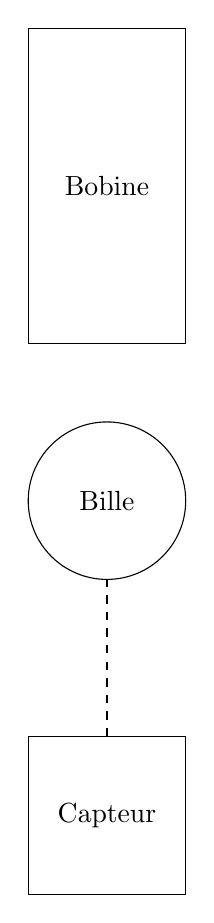
\begin{tikzpicture}[x=5mm,y=5mm]
        \node[rectangle,draw,minimum width = 20mm,minimum height = 40mm,anchor=center] (BO) {Bobine};
        \node[circle,draw,minimum width = 20mm,minimum height = 20mm,anchor=center] at (0,-8) (B) {Bille};
        \node[rectangle,draw,minimum width = 20mm,minimum height = 20mm,anchor=center] at (0,-16) (SH) {Capteur};
        \draw [shorten >=0pt,dashed] (SH)--(B);
    \end{tikzpicture}
\end{center}


\section{Début du projet}
Nous avons commencé par nous familiariser avec le matériel à disposition :
\begin{itemize}
    \item Une bobine avec noyau mobile
    \item Une bille en acier d'environ 35,8g
    \item Un portique pour installer la bobine
\end{itemize} 
Nous avons donc installé la bobine sur le portique et utilisé l'alimentation DC en mode CC/CV pour régler le courant dans la bobine. Cela a pour effet de créer un champ magnétique plus ou moins fort qui attire la bille vers le noyau de la bobine. Nous avons donc mesuré le courant nécessaire pour que la bille décolle pour différentes distances, de 1mm à 23mm. Nous obtenons le tableau suivant : \newline

\begin{center}
    \begin{tabular}{|c|c|c|r|l}
    \cline{1-4}
    Tension & Courant & Distance minimale bille & \multicolumn{1}{c|}{$R_{bobine}$} &  \\ \cline{1-4}
    8,612   & 0,647   & 1mm                     & 13,31$\Omega$                        &  \\ \cline{1-4}
    11,296  & 0,847   & 5mm                     & 13,34$\Omega$                        &  \\ \cline{1-4}
    13,96   & 1,047   & 8mm                     & 13,33$\Omega$                        &  \\ \cline{1-4}
    16,623  & 1,247   & 14mm                    & 13,33$\Omega$                        &  \\ \cline{1-4}
    19,293  & 1,447   & 15mm                    & 13,33$\Omega$                        &  \\ \cline{1-4}
    21,962  & 1,647   & 19mm                    & 13,33$\Omega$                        &  \\ \cline{1-4}
    24,65   & 1,847   & 20mm                    & 13,35$\Omega$                        &  \\ \cline{1-4}
    27,34   & 2,047   & 22mm                    & 13,36$\Omega$                        &  \\ \cline{1-4}
    29,915  & 2,247   & 23mm                    & 13,31$\Omega$                        &  \\ \cline{1-4}
    \end{tabular}
\end{center}
Graphique :
\begin{center}
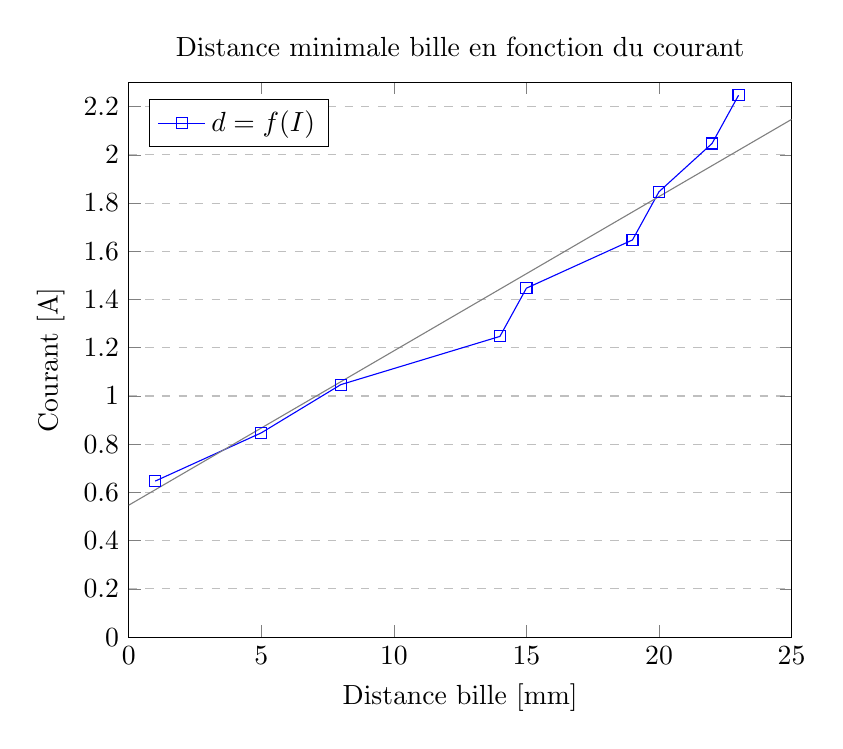
\begin{tikzpicture}
    \begin{axis}[
        title={Distance minimale bille en fonction du courant},
        xlabel={Distance bille [mm]},
        ylabel={Courant [A]},
        xmin=0, xmax=25,
        ymin=0, ymax=2.3,
        xtick={0,5,10,15,20,25},
        ytick={0,0.2,0.4,0.6,0.8,1,1.2,1.4,1.6,1.8,2,2.2,2.4},
        legend pos=north west,
        ymajorgrids=true,
        grid style=dashed,
    ]
    
    \addplot[
        color=blue,
        mark=square,
        ]
        coordinates {
        (1,0.647)(5,0.847)(8,1.047)(14,1.247)(15,1.447)(19,1.647)(20,1.847)(22,2.047)(23,2.247)
        };
        \legend{$d = f(I)$}
    
    \addplot[color=gray, mark=none] coordinates {(0,0.547)(25,2.147)};
        
    \end{axis}
    \end{tikzpicture}
\end{center}

\section{Idée : pilotage de l'alimentation par USB}
Dans l'optique de réguler la distance entre la bille et la bobine, il faut pouvoir contrôler le courant traversant la bobine. Nous avons donc eu l'idée d'essayer de contrôler l'alimentation de la salle de TP avec le port USB situé à l'arrière de celle-ci. En effet, si cette méthode est convaincante, il suffirait d'acquérir la tension du capteur Sharp avec un ADC (Analog to Digital Converter) et un algorithme de type PID permettrait de corriger la position de la bille (solution numérique donc). \newline

Nous avons donc cherché le manuel de l'alimentation RIGOL afin de comprendre comment lui envoyer des requêtes. Il faut en fait utiliser des instructions SCPI \texttt{(Standard Commands for Programmable Instruments)} pour communiquer avec l'alimentation. Par exemple, la commande \texttt{:INST CH1 } permet de choisir le canal à utiliser (de CH1 à CH3) et \texttt{:CURR 0.4} permet de définir la limite de courant à $0,4A$. \\
Au début, nous rentrions les commandes à la main dans le logiciel de l'alimentation :
\begin{center}
    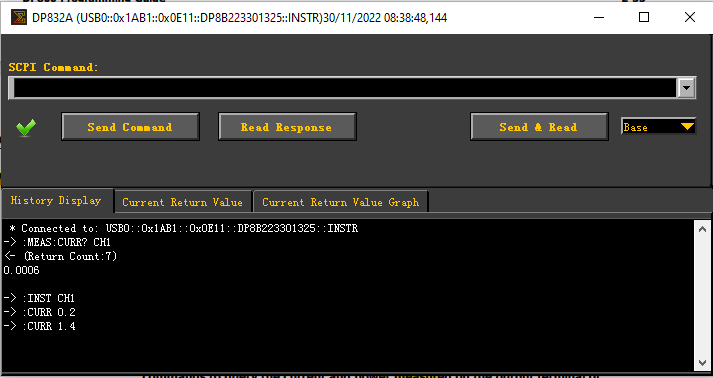
\includegraphics[width=0.5\textwidth]{picture/ultra_sigma_control_panel_exemple of command.PNG}
\end{center}
Cependant, nous avons vite compris que cela n'était pas très pratique. Nous avons donc décidé d'utiliser un script Python pour envoyer les commandes à l'alimentation. Nous avons utilisé la librairie \texttt{PyVISA} pour communiquer avec l'alimentation. Voici un exemple de script Python qui permet de changer la limite de courant toutes les secondes :
\begin{lstlisting}[language=python]
    import pyvisa
    import time

    resources = pyvisa.ResourceManager()
    
    psu = resources.open_resource(resources.list_resources()[0])
    psu.write(":INST CH1")
    while 1:
        psu.write(":CURR 0.4")
        time.sleep(1)
        psu.write(":CURR 0.2")
        time.sleep(1)
\end{lstlisting}
Voyant que la commutation entre les deux valeurs de courant pouvait être rapide, nous avons voulu utiliser l'oscilloscope pour vérifier la qualité de l'asservissement de l'alimentation. Voici le résultat (tension en jaune, courant en bleu) :
\begin{center}
    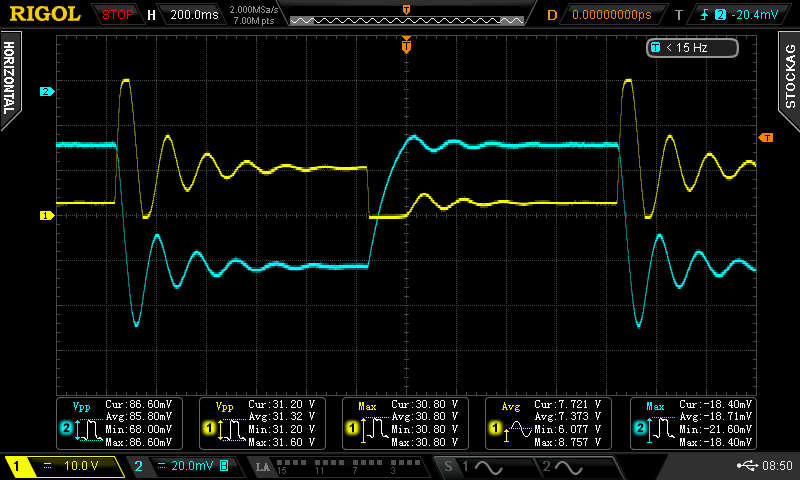
\includegraphics[width=1\textwidth]{picture/oscillo_bleu_courant_jaune_tension_avec_execution_python_program.png}
\end{center}
On remarque que la commutation se fait bien mais qu'il y a trop d'oscilations. Cela pourrait causer la chutte de la bille. Nous ne pouvons donc pas utiliser cette méthode pour contrôler le courant de la bobine. Nous avons aussi essayé de contrôler la tension de l'alimentation mais les résultats sont similaires.
\newpage
\section{Etude du capteur Sharp}
Afin de déterminer la distance entre la bille et la bobine, nous avons utilisé un capteur Sharp GP2Y0A21YK0F. Ce capteur est un capteur de distance infrarouge qui renvoie une tension représentant la distance entre le capteur et un obstacle. Nous avons donc mesuré la tension de sortie du capteur à l'aide du multimètre et nous avons fait varier la distance entre la bille et le capteur (pas de 0,5mm). Comme la distance entre un obstacle et le capteur est comprise entre 4 et 8mm, nous avons décidé de faire une régression linéaire sur les points de la courbe entre 4 et 8cm. Voici le résultat :
\begin{center}
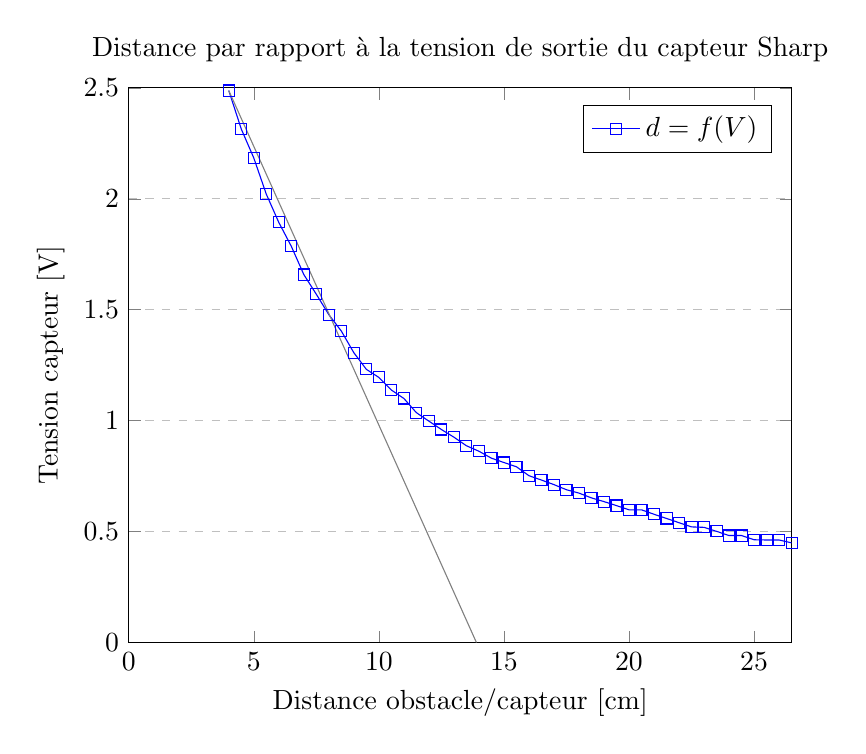
\begin{tikzpicture}
    \begin{axis}[
        title={Distance par rapport à la tension de sortie du capteur Sharp},
        xlabel={Distance obstacle/capteur [cm]},
        ylabel={Tension capteur [V]},
        xmin=0, xmax=26.5,
        ymin=0, ymax=2.5,
        xtick={0,5,10,15,20,25},
        ytick={0,0.5,1,1.5,2,2.5},
        legend pos=north east,
        ymajorgrids=true,
        grid style=dashed,
    ]
    
    \addplot[
        color=blue,
        mark=square,
        ]
        coordinates {
        (4,2.4878)(4.5,2.3145)(5,2.1841)(5.5,2.021)(6,1.8936)(6.5,1.7859)(7,1.6585)(7.5,1.5697)(8,1.4778)(8.5,1.4037)(9,1.3062)(9.5,1.2312)(10,1.1949)(10.5,1.138)(11,1.100)(11.5,1.036)(12,0.9978)(12.5,0.96)(13,0.9255)(13.5,0.8869)(14,0.8621)(14.5,0.8308)(15,0.8112)(15.5,0.7921)(16,0.7518)(16.5,0.7322)(17,0.7116)(17.5,0.6885)(18,0.6734)(18.5,0.6517)(19,0.635)(19.5,0.6171)(20,0.598)(20.5,0.598)(21,0.578)(21.5,0.559)(22,0.54)(22.5,0.521)(23,0.519)(23.5,0.501)(24,0.482)(24.5,0.482)(25,0.463)(25.5,0.462)(26,0.462)(26.5,0.449)
        };
        \legend{$d = f(V)$}
    
    \addplot[
        color=gray,
        mark=none,
        ]
        coordinates {
        (4,2.4878)(13.9,0)
        };

    \end{axis}
    \end{tikzpicture}
\end{center}
On obtient donc le modèle linéaire suivant : $d = -4,10u + 13,9$ avec $d$ en cm et $u$ en V. 

\section{Mesure des caractéristiques de la bobine}
Avec nos mesures en courant continu, nous avons pu déterminer la résistance interne de la bobine. Celle-ci vaut en moyenne $13,33\Omega$. Afin de déterminer l'inductance réelle de la bobine, nous avons utilisé le générateur basse fréquence (amplitude de 1,6V crête, fréquence de 2Hz) pour identifier le déphasage induit par la bobine à l'aide de l'oscilloscope (environ 60ms ou $-0,75 \text{ rad}$). Calculons l'inductance de la bobine :
\begin{align*}
    Z &= R + jL\omega = 13,33 + jL\omega \text{ et } \arctan\left(\dfrac{L\omega}{R}\right) = 0,75 \\
    L &= \dfrac{R\tan(0,75)}{\omega} = 0,98\text{ H}
\end{align*}


\section{Détermination de la fonction de transfert}
A l'aide d'Hopkinson, nous avons pu déterminer l'inductance L en fonction de la position de la bille : $L(z) = L_0 + \dfrac{L_1}{1+\alpha z}$. Nous avons déjà déterminé la valeur de $L_0 = 0,98H$ (inductance de la bobine sans bille). En appliquant le principe fondamental de la dynamique, nous avons :
\begin{align*}
    \overrightarrow{F} + \overrightarrow{P} &= m\overrightarrow{a} \\
    \text{Sur l'axe \overrightarrow{z} : } -F(z) + mg &= m\ddot{z} \\
\end{align*}
On remarque que l'équation différentielle n'est pas linéaire :
\begin{align*}
    \dfrac{I^2L_1\alpha}{2(1+\alpha z)^2} + mg &= 0
\end{align*}
On linéarise avec Taylor autour de $(z_0, I_0)$ : 
\begin{align*}
    F(z, I) &\approx F(z_0, I_0) + \dfrac{dF}{dz}(z-z_0) + \dfrac{dF}{di}(I-I_0)
\end{align*}
On note $\dfrac{\partial F}{\partial I} = \dfrac{I_0L_1\alpha}{(1+\alpha z_0)^2} = k_i$ et $\dfrac{\partial F}{\partial z} = \dfrac{I_0^2L_1\alpha^2}{(1+\alpha z_0)^3} = -k_z$\\
En choisissant $z_0$ quand la bille est à l'équilibre, on a $F(z_0, I_0) + mg = 0$, la force magnétique compense le poids de la bille. On a donc :
\begin{align*}
    \dfrac{I_0^2L_1\alpha}{2(1+\alpha z_0)^2} &= mg \\
\end{align*}
Nous pouvons maintenant utiliser les mesures effectuées au début du projet (distance minimale pour le décollage de la bille par rapport au courant) pour trouver $L_1$ et $\alpha$. En linéarisant, on obtient $a = \sqrt{\dfrac{L_1}{2\alpha mg}}$ et $b = \dfrac{1}{\alpha}$. On utilise Regressi pour trouver les valeurs de $a$ et $b$ :
\begin{align*}
    a &= 0,0682 \\
    b &= 0,485
\end{align*}
Donc $L_1 = 6,73H$ et $\alpha = 2,06$ et $L(z) = 1 + \dfrac{6,73}{1+2,03z}$. \\
Ainsi, on a $F(z, I) \approx F(z_0, I_0) + k_i(I-I_0) - k_z(z-z_0) \approx F(z_0, I_0) + k_iI - k_zz$ car $z \approx z_0$ et $I \approx I_0$.
Donc on a :
\begin{align*}
    mg - F(z_0, I_0) - k_iI + k_zz &= m\ddot{z} \\
    -k_iI(t) + k_zz(t) &= m\ddot{z} \text{ car } mg - F(z_0, I_0) = 0\\
\end{align*}
On applique la transformée de Laplace :
\begin{align*}
    -k_iI(p) = (k_z + mp^2)z(p)
\end{align*}
On obtient donc la fonction de transfert :
\begin{align*}
    H(p) = \dfrac{z(p)}{I(p)} = \dfrac{-1}{-\dfrac{k_z}{k_i}+\dfrac{mp^2}{k_i}}
\end{align*}

\end{document}